\documentclass[a4paper,11pt]{scrartcl}

\usepackage[T1]{fontenc}
%\usepackage[utf8]{inputenc}
\usepackage{lmodern}

\usepackage[english]{babel}
\usepackage{graphicx}
\usepackage{amsmath,bm}
\usepackage[dvipsnames]{xcolor}
\usepackage{hyperref}
\hypersetup{
  colorlinks=true,
  urlcolor=blue,
  linkcolor=Mahogany,
  citecolor=BurntOrange
}
\usepackage[small,sf]{caption}
\usepackage{booktabs}
\usepackage{listings}
\usepackage{units}
\usepackage{wrapfig}
\usepackage{amsmath}
\usepackage{url}  % \path{} allows linebreaks
\usepackage{mathrsfs}
\usepackage{wrapfig}


\def\td{\$HandsOn/tutorial\_4}
\def\sd{\$HandsOn/tutorial\_4/scripts}

\def\IPI{i-pi input.xml}
\def\FHI{aims.ipi.x}

\usepackage{subfigure}

\usepackage{verbatim}
\usepackage{multirow}
\usepackage[dvips]{geometry}
\geometry{textwidth=15cm,textheight=24cm,top=3.5cm}

\setlength{\parindent}{24pt}
\setlength{\parskip}{1.0ex plus 0.5ex minus 0.2ex}

% \setlength{\footnotemargin}{0.6em}
\setcounter{secnumdepth}{0} % no section numbering

\lstset{
    basicstyle=\ttfamily,
    keywordstyle=\color{BrickRed},
    commentstyle=\color{Gray},
    stringstyle=\color{black},
    emphstyle=\color{RedOrange},
    columns=flexible,
    showstringspaces=false,
    xleftmargin=1em,
    deletekeywords={bin,all}
}


\lstdefinelanguage{Bash}
{
   alsodigit={-,.},
   morekeywords={ cp2k.popt, lmp_ubuntu, i-pi, vmd, done, python, mpirun, touch, tail, trajworks, autocorr, awk, i-pi-mergebeadspdb, grep, head, cp, cd, cat, ls, pwd, bash, sed, mkdir, vi, sh}
   %morecomment=[s][\color{orange}]{#}{\}
}

\newcommand{\mr}[1]{{\color{purple}{#1}}}


\begin{document}

%%%%%%%%%%%%%%%%%%%%%%%%%%%%%%%%%%%%%%%%%%%%%%%%%%
% Titel page
%%%%%%%%%%%%%%%%%%%%%%%%%%%%%%%%%%%%%%%%%%%%%%%%%%
\thispagestyle{empty}
\begin{center}\huge\bfseries
  \rule{1.0\textwidth}{1pt}
 A Short Tutorial on Ab Initio Molecular Dynamics and Path Integral Molecular Dynamics \\
% Accuracy, Efficiency and Reproducibility in Computational Materials Science\\
[0.5em] Using the i-PI/FHI-aims Infrastructure (2018)
  \rule{1.0\textwidth}{1pt}
\end{center}
\vfill
\begin{center}\LARGE\bfseries
  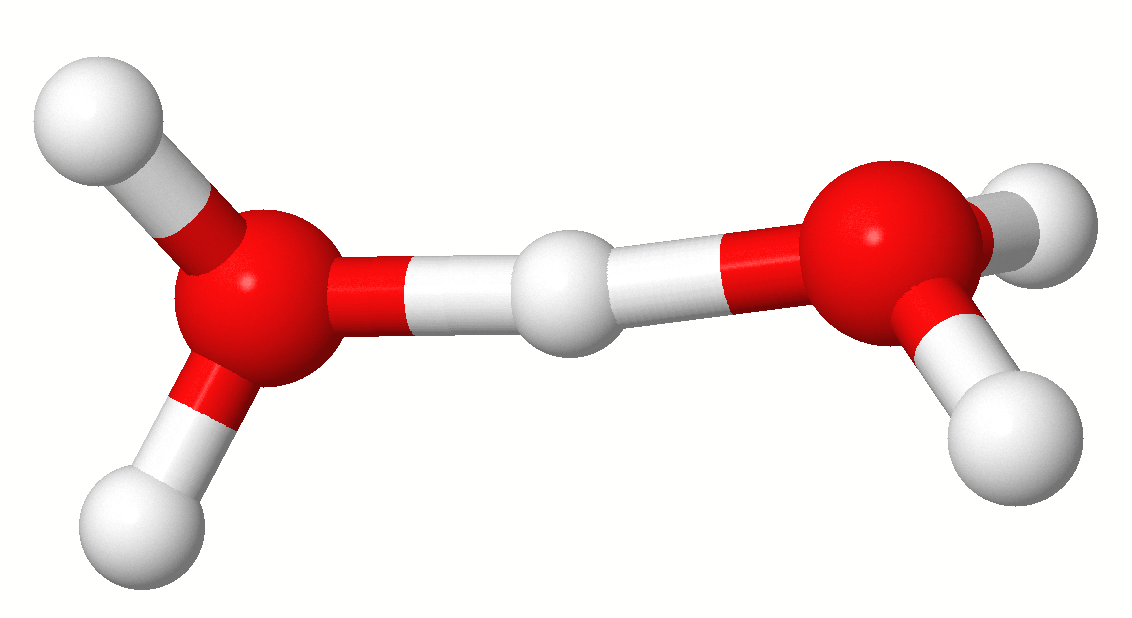
\includegraphics[width=0.5\textwidth]{H5O2.png}
  \vfill\vfill
 (\textit{Ab initio}) Molecular Dynamics\\
  Manuscript for Exercise Problems
\end{center}
\vfill
\begin{center}\large\bfseries
  \rule{1.0\textwidth}{1pt}
  \vfill
  Prepared by Yair Litman, Nathaniel Raimbault and Mariana Rossi\\[0.4em]
\end{center}

\clearpage


%/usr/local/aimsfiles/scripts
%/usr/local/aimsfiles/tutorial4


% \title{Practical session: \textit{Ab initio} Molecular Dynamics}
% \author{\large{Prepared by Mariana Rossi, Carsten Baldauf, and Luca M. Ghiringhelli}}
%
% \date{\today}
% %\date{Friday, June 26 2009, 14:00}
%
%
% %\begin{abstract}
% %\end{abstract}
%
% \maketitle

% \begin{figure}[ht]
% \begin{center}
% 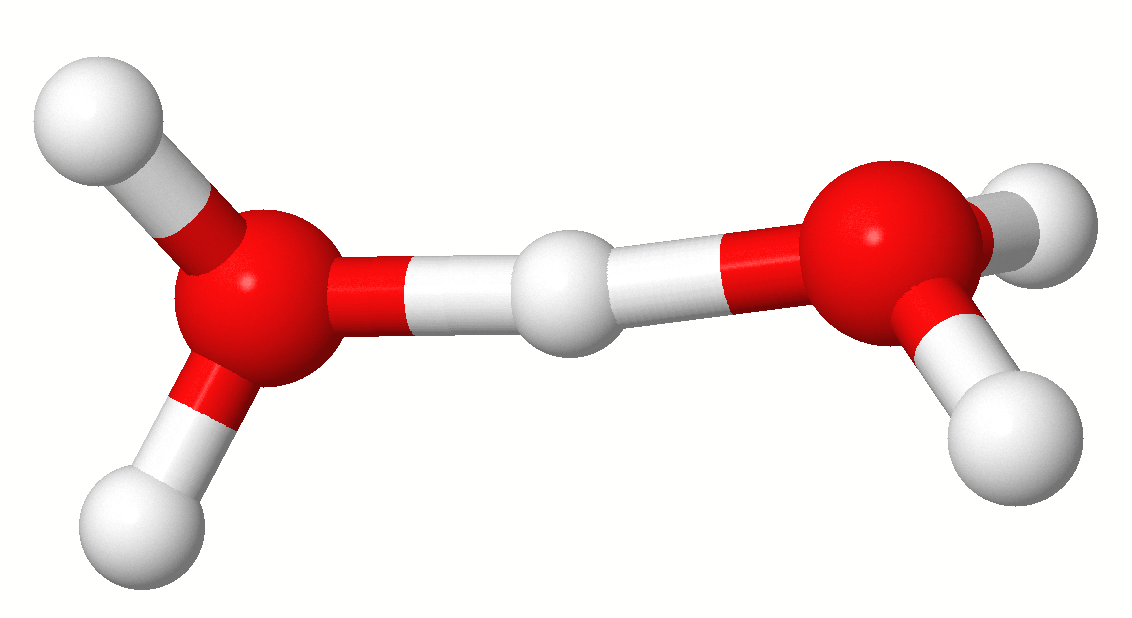
\includegraphics[width=0.4\textwidth]{H5O2}
% %\includegraphics[width=0.35\textwidth]{ch3-dimer.png}
% \caption{The Zundel cation, H$_5$O$_2^+$.}
% \end{center}
% \end{figure}

%%%%%%%%%%%%%%%%%%%%%%%%%%%%%%%%%%%%%%%%%%%%%%%%%%
% Introduction
%%%%%%%%%%%%%%%%%%%%%%%%%%%%%%%%%%%%%%%%%%%%%%%%%%
\section{Introduction}
\par
	With this tutorial, we aim at introducing you to techniques used to solve the classical equations of motion for a system of interacting particles. 
The strategy we adopt is molecular dynamics (MD), a method that can be considered as old as modern physics itself, since in this framework one {\em propagates}  in time a system of particles, given initial positions and momenta, by numerical integration of Newton's equations of motion. 
This technique allows one to sample the potential energy surface of a system at constant energy (microcanonical ensemble) and at constant temperature (canonical ensemble). As long as the {\em ergodic hypothesis} is valid, we will be, in principle, able to relate the time averaged parameters (or properties), to the thermodynamic averages over the corresponding statistical ensemble. 

The kind of MD we are interested in is Born-Oppenheimer MD, where the degrees of freedom of the nuclei are considered to be decoupled from the degrees of freedom of the electrons (Born-Oppenheimer approximation). On top of this approximation, usually one treats the nuclei as classical particles. Therefore, the forces between them are evaluated by solving the (ground-state) electronic structure problem for a given number of electrons and for a given position of the nuclei. 
In this tutorial, the electronic structure problem is solved via Density Functional Theory (DFT) within the FHI-aims code and the nuclei problem is managed by  the i-PI \cite{ipi} code. i-PI works through a client-server paradigm, where the \textit{ab initio} code, in this case FHI-aims, is the client that provides the calculation of interatomic forces, and i-PI is the server that provides the evolution of the equations of motion that sample the desired ensemble. 

By the end of the tutorial, we will also show a small example on how one can also treat the nuclei as quantum particles, by performing what we call ``path-integral molecular dynamics'' (PIMD). This type of dynamics is
based on the Feynman path integral formalism \cite{Feynman}. This 
formalism exploits the isomorphism between the partition function of a quantum particle with that of 
several repeated classical particles (beads) connected by harmonic springs and forming a closed 
loop (ring polymer). In PIMD, molecular dynamics is employed to drive phase-space statistical sampling. Static 
ensemble properties of the system can be accurately (in principle exactly in the limit of infinite beads) evaluated within this technique. 

All the necessary theoretical background for a good understanding of this tutorial is given in the lectures of Luca Ghiringhelli (about statistical mechanics) and Mariana Rossi (about \textit{ab initio} molecular dynamics).

The tutorial contains five exercises. All of them are based on a paradigmatic system, namely the gas-phase (isolated) H$_5$O$_2^+$, which some of you may recognize as the Zundel (cat)ion. 
%This system is one of the (protonated) water clusters that are thought to be the ``building blocks'' of liquid water \cite{tuckerman}.\\


The \textbf{first}, and quick, introductory exercise presents the machinery we will use through the tutorial. 
In particular, you will learn how to setup the i-PI and FHI-aims inputs.


The \textbf{second} and \textbf{third} exercises pose the problem of choosing the right settings for obtaining a stable and reliable molecular dynamics trajectory.
In particular we will investigate the effect of the self-consistent cycle and force convergence thresholds as well as the influence of the size of the time step. \\

The \textbf{fourth} exercise deals with the choice of a thermostat for simulating the canonical ensemble, i.e., the contact between your system of interest and a thermal reservoir. 
In this tutorial we will focus on the so-called stochastic thermostats. Other implementations, for example based on extended Lagrangians exist as well, and will be briefly explained in the exercise.
Also, we will see how one can use thermostats to break the fluctuation dissipation theorem and mimic the quantum nature of the nuclei by changing the momentum distribution on a ``classical-nuclei'' simulation.
%Many traditional thermostats are implemented in i-PI, but for this tutorial we will focus only on xxxxxxxxx.
 %and the colored-noise thermostats.  The latter opens the possibility for accurate inclusion of quantum statistics for nuclei, whereas the usual MD machinery treat them as classical particles.


In the  \textbf{fifth} and last exercise we will compute free energy differences through the method of thermodynamic integration. In addition, we are going to compare results obtained from simulations that neglect quantum statistics for the nuclei with results from simulations that take into account these effects (PIMD). 

%\vspace*{24pt}

%\colorbox{Melon}{\frame{\begin{minipage}[r]{0.95\textwidth}
%\begin{center}
%\vspace{0.3cm}
%\hspace{4pt} All the useful files for this tutorial (together with solutions) are located in:\\
%\vspace{0.3cm}
%\hspace{12pt} \texttt{\td} 
%\vspace{0.3cm}
%\end{center}

%\hspace{6pt} You can find the solutions in:
%\hspace{12pt} \texttt{\$HandsOn/tutorial\_4/Solutions} 
%\end{minipage}}}

\newpage
\section*{Molecular Dynamics: a client/server approach}

{\large\textbf{Exercise 1: Getting started}}

In this exercise we are going to familiarize ourselves with the important notations of
i-PI input files. As mentioned previously, the i-PI program works through a client-server architecture.
i-PI is a python code, and as such does not to be explicitly installed in the machine. It relies on
the python and numpy being preinstalled. The code can be downloaded from \href{http://ipi-code.org/}{http://ipi-code.org/}, where one can find
also more information regarding the whole project.
It can use INTERNET or UNIX sockets, that allow the system to be simulated
on the same machine or on a different machine, as long as the calculation can communicate with the server.


 Let's take a look at the input files.
The example simulation here will consist of one zundel molecule in the canonical (NVT) ensemble at 300K.

\textit{Server:} An example of an input file for i-PI can be found in \texttt{exercise\_1/input.xml}. It is an xml file, which is quite intuitive to learn.
% The input is not complete.
 Please take your time to understand the keywords that are there and consult the i-PI manual, contained in the i-PI program package.
%There is only one  field that should be completed in the file: the field address about the socket communication.
We will be using UNIX sockets here, which is the most convenient way to use the code when running both servers and clients
in small desktop (or laptop) machines. For that, we have to specify only the \texttt{<address>}, which can simply be a string containing a name of your choice. For internet sockets, one would have to provide
the relevant IP address for the  \texttt{<address>} field and a number for the \texttt{<port>} field. For example, if server and client would run in the same machine,
one could set the mode of \texttt{<ffsocket>} to \texttt{inet} and write \texttt{localhost}  in the address field. In HPC architecture this
procedure can be more involved as often computing nodes do not have a network connection to the head node, or one cannot keep a program running 
in the head node for indefinite amounts of time. Solutions can be found through scripts that write the address on the relevant files
only after a job starts running in a specific computing node, or through setting up tunnels to other machines.
If you can't find a solution to your problem, do no hesitate to ask in the i-PI forum: \href{http://ipi-code.org/resources/forum/}{http://ipi-code.org/resources/forum/}.  
% Just write in the \texttt{<address>} field a string of your choice, e.g. \texttt{Berlin-2017-H5O2}.

%We will be using UNIX domain sockets here, since we will be running both server and client in the same machine. Just write in the \texttt{<address>} field a string of your choice, e.g. \texttt{Berlin-2017-H5O2}.

%\footnote{
%(In the input there is a commented block with an example of how it would look if we would use internet sockets communicating with the localhost. If using in different machines or nodes, one would have to give a proper IP address at the "address'' field.}


%More detailed instructions about the input file can be found in manual of i-PI.

\textit{Client:} The keyword to add to the \texttt{control.in} file of FHI-aims is

\texttt{use\_pimd\_wrapper UNIX:<address> <portnumber>} 
 
\noindent where \texttt{<address>} should be substituted by the name of the socket you choose, and the port can be any number since it does not play a role for UNIX sockets.
% Since we are using \textbf{UNIX domain sockets, one can just put a dummy number on the \texttt{portnumber} field}. 
%Since we are using INTERNET socket, both fields \texttt{hostaddress} and  \texttt{portnumber} in the \texttt{control.in} file should match the ones
%in the \texttt{input.xml} file. 
The address that goes in the \texttt{control.in} file should match the one in the \texttt{input.xml} file of i-PI.
The \texttt{geometry.in} is only provided for the initialization of FHI-aims, so in order to avoid inconsistency problems always check that the atoms are listed in the same order as in the i-PI input file.
(Here, we did that for you ;) )

\textit{Note that in all subsequent exercises you will be free to choose \texttt{<address>} as you want, and you should please change it in your input files (\texttt{control.in} and \texttt{input.xml}) so that your server and your client always match!}

% Since we are using \textbf{UNIX domain sockets, one can just put a dummy number on the \texttt{portnumber} field}. In the \texttt{hostaddress}  field write, for example, \texttt{Berlin-2017-H5O2}. The \texttt{geometry.in} is only provided for the initialization of FHI-aims, so in order to avoid convergency problems be sure the atoms are listed in the same order as in the i-PI input file.

Let's run an i-PI+FHI-aims Molecular Dynamics simulation!


\noindent{\textbf{Instructions}}
\begin{itemize}
 \item Open a terminal at the current directory and launch i-PI by typing
 \begin{center}
   \texttt{\IPI}
\end{center}

 At this point i-PI should start and parse the input file. At the bottom of the
output on the screen it should say:

\begin{lstlisting}[language=bash]
Created unix socket with address EX1
@ForceField: Starting the polling thread main loop.
\end{lstlisting}
This means i-PI has started properly, has created the UNIX socket, and is
waiting for the communications from the clients that take care of the force evaluations.

 \item Now we can launch FHI-aims. Open a second terminal, either
manually or by typing Ctrl+Shift+t, and enter the command
 
 \begin{center}
   \texttt{\FHI}
\end{center}

Then FHI-aims should start and you will see some outputs.

\item

Now switch to the terminal where i-PI is running, notice that i-PI has built
the connection with FHI-aims with the following message,

\begin{lstlisting}[language=bash]
 @SOCKET:   Client asked for connection from . Now hand-shaking.
 @SOCKET:   Handshaking was successful. Added to the client list.
\end{lstlisting}

and started the Molecular Dynamics simulation. It should also print on screen some
information about the time cost of each MD step.

\item What we are going to do now is to kill FHI-aims (don't worry, you shall not be sued for that). 
Simply switch to the terminal where FHI-aims is running and press Ctrl+c. Now look at whether i-PI
is still running. Notice that although the evolution of the MD is paused, i-PI itself
does not die off but instead continues to run and waits for a new client to take
over. Now start FHI-aims again by typing:

 \begin{center}
   \texttt{\FHI}
\end{center}


What happens to i-PI now?

\item What if one stops i-PI? Kill i-PI by typing Ctrl+c where it is running, or
create a file named EXIT in the folder where i-PI is running (you can use the
bash command  \texttt{touch EXIT}). Watch how i-PI responds, and how FHI-aims
reacts. Think about what are the advantages of a clean exit when a MD
program stops unexpectedly.

\item Take a look at all the output files written by i-PI. You should have the file ex1.out that describes the system properties, ex1.pos.xyz that records
the atomic trajectories, and RESTART that contains all the information to
restart the simulation.

\item Last (and tricky) question , we are dealing with a charged system. Can you find where the total charge in the input.xml file is specified? 
Why?
\end{itemize}
 
\textit{Timing:  $\sim$20 minutes total}

\newpage
\section*{The microcanonical ensemble}

%\begin{enumerate}
{\large\textbf{Exercise 2: The importance of the SC convergence criteria}}

In this exercise, we will investigate the importance of the self-consistency convergence criteria
when simulating the microcanonical ensemble. The the input files for i-PI can be found in the folder \texttt{exercise\_2}. 
Please note that the initialization in i-PI is done with a previously thermalized geometry.

\noindent{\textbf{Instructions}}

\begin{itemize} 
\item First, build an input file (\texttt{control.in}) for FHI-aims using the LDA (\textbf{pw-lda}) functional, no spin polarization (\textbf{spin none}), and using the ``\textbf{light}'' numerical and basis set standards for the species. 
Add the line corresponding to the i-PI communication that was shown in the previous exercise, as well as the following line to tell FHI-AIMS that you need to compute the forces:
\begin{center}

\texttt{compute\_forces .true.}
\end{center}
Please refer to the manual for the exact syntax of these flags.  

Do not add any flags that we do not mention. They are not needed and might hinder the performance of the calculation. 

\item We want to run a 0.15ps MD run in the microcanonical ensemble (NVE), using a 0.0005ps ($\Delta t = 0.5$fs) time step. 
For that, open the provided \texttt{input.xml} and change the lines \texttt{timestep} and \texttt{total\_steps}  accordingly. 
%In addition note that we have specified the \texttt{dynamics} mode to be `nve'. 
You also need to specify the \texttt{dynamics} mode to be 'nve'.
The file chosen for the \texttt{initialization} is a checkpoint file containing positions, velocities, and
some other settings from a previous
simulation where this molecule was thermalized, using the `nvt' mode \footnote{You will see how such a thermalization is done in \texttt{exercise 4}.} -- that is what the  `chk'  mode in i-PI means \footnote{You can open and read the checkpoint file if you wish in order to see the structure of it, which is actually also an .xml file very similar to the input of i-PI but containing more blocks.}.  
In this case, initializing from the checkpoint file means that i-PI will read positions and velocities from it.  


\item After everything is set up, start the simulation in the following way

%{\bf WARNING:} ``Light'' self-consistency settings just refers to the four tags given
%above, and {\bf not} at all to any settings regarding the basis set. So please do not
%change the provided settings for the basis set.

\vspace{0.3cm}
\colorbox{Peach}{\frame{\begin{minipage}[r]{0.95\textwidth}
\vspace{0.3cm}
\begin{center}
In order to start  the simulation type:\\

\vspace{0.3cm}
\texttt{\IPI \, >  output-i-PI \&}\\
\vspace{0.3cm}
(Wait 5 seconds in order to let i-PI do the initialization)\\
\vspace{0.3cm}
\texttt{mpirun -np 8  aims.ipi.x > output-FHI-aims \&}

\begin{itemize}
\item The symbol \texttt{\&} puts the run in the background, so that the output file is created, but the terminal is free for other use.
\item If you would like anyway to have a dynamic view of what happens in your output, after starting the simulation you can type:

\texttt{tail -f <name-of-output>} \\
Press Ctrl+c to exit.

\item ATTENTION: do not start another FHI-aims run simultaneously. \\That would slow down BOTH calculations considerably.
\end{itemize}
\vspace{0.3cm}
\end{center}
\end{minipage}}}

\vspace{0.3cm}

\item When the previous calculation is over, run another simulation, keeping all parameters
mentioned above but changing the name of the output and also changing
to the following ``loose'' self-consistency convergence criteria:

\begin{center}

\texttt{sc\_accuracy\_rho  1E-2}

\texttt{sc\_accuracy\_eev  1E-1}

\texttt{sc\_accuracy\_etot 1E-2}

\texttt{sc\_accuracy\_forces 1E-1}
\end{center}

\item Finally, run another simulation with ``accurate'' self-consistency criteria:

\begin{center}
\texttt{sc\_accuracy\_rho  1E-5}

\texttt{sc\_accuracy\_eev  1E-4}

\texttt{sc\_accuracy\_etot 1E-6}

\texttt{sc\_accuracy\_forces 5E-4}
\end{center}
\textbf{IMPORTANT}: Remember to change the output prefix in the i-PI input in order to not overwrite any output file.
\vspace{0.1cm}\\
\textbf{REMINDER}: Choose \texttt{<address>} in your input files (\texttt{control.in} and \texttt{input.xml}) so that your server and your client  match.

\vspace{0.1cm}
When it is done, plot the total energy (\texttt{conserved} in the i-PI language for NVE. Why?)  vs. the simulation time in \texttt{xmgrace}.
\footnote{If you are more confortable with, e.g., \texttt{gnuplot}, please feel free to use it instead!}

For a short guide on how to plot files with multiple columns in \texttt{xmgrace}  see the Appendix to	 this tutorial.

Can you see how the energy drifts with the ``loose'' settings? Find out what were the the default criteria for these thresholds that were applied in the first simulation of this exercise (hint: you can find them in the FHI-aims output). How do they compare with the ``loose'' and ``accurate'' settings with respect to this energy drift? 


\end{itemize}

\vspace{0.4cm}
Ideally, there should be no energy drift, since the energy is conserved in the microcanonical ensemble.
 The reason for this drift is that we leave the true Born-Oppenheimer surface if we don't converge well our 
electronic structure; this leads to an unphysical (and undesirable) energy drift.

\textit{Timing:  $\sim$20 minutes total}

\clearpage


{\large\textbf{Exercise 3: The importance of the time step size}}

Here, we will investigate the effects of the time step size for the integration of the
equations of motion in a microcanonical molecular dynamics simulation.
For a better illustration, we will not only consider the H$_5$O$_2^+$ molecule, but also its heavier,
deuterated counterpart D$_5$O$_2^+$ \footnote{The deuterium atom has one proton and one neutron in its nucleus,
thus about twice as heavy as hydrogen.}.


Checkpoint files for both H$_5$O$_2^+$ and D$_5$O$_2^+$ from 
previous simulations where the molecules were thermalized are provided in the folder \texttt{exercise\_3}.
Use the same \texttt{control.in} (the ``accurate'' one) and  \texttt{geometry.in} from the previous exercise 
Both H$_5$O$_2^+$ and D$_5$O$_2^+$ have the exact same electronic structure. This means that for converging the DFT self consistent cycle, the answer will
be the same no matter the name or mass of the nuclei \footnote{In extreme cases changing the mass of the nuclei could have an effect, but it is not the case for just the addition of one neutron.}.
Therefore, one can use the same FHI-aims input files for both molecules. What will matter, though, is that in the evolution of the nuclei through Newton's equation of motion, the mass of the atom
enters in the definition of the force and the propagation of the equations of motion. Therefore we will use different masses (corresponding to hydrogen and deuterion) in the checkpoint file that i-PI is
reading in to initialize. If you wish to have a look at where this is specified, open that file and look for the block named \texttt{<m shape=... >} in which the units are atomic mass units.


An \texttt{input.xml} file is also provided. Please read and complete it in a appropriate way for each of the following tasks.


In order to speed up the exercise, each group will simulate either H$_5$O$_2^+$ or D$_5$O$_2^+$.
The suggested choice of the molecule will be made clear (announced) by the tutors at hand.

%The species default for deuterium, that you should put in your \texttt{control.in} file, is provided
%in this exercise's folder. The suggested choice of the molecule will be made clear (announced) by the tutors at hand.



\noindent{\textbf{ Instructions}}
\begin{itemize}

\item Copy the "accurate" \texttt{control.in}  and  the \texttt{geometry.in} files from the last exercise.

Do not add any flags that we do not mention! They are not needed and might hinder the performance of the calculation.

\item Modify the \texttt{input.xml} file to run  a 0.40\,ps MD run in the microcanonical ensemble, using a 0.0005\,ps ($\Delta t = 0.5\,$fs) time step and run it \footnote{Hint: There should be 800 steps.}. 

\item When it is done, plot the total energy  vs. the simulation time  with \texttt{xmgrace}.

\item Increase the time step to $0.001\,$ps and run the simulation again, take the necessary precautions to not overwrite the files.

\item Increase the time step to $0.002\,$ps and run the simulation again, take the necessary precautions to not overwrite the files. If FHI-aims aborts the run,  you can create a file named EXIT in the folder where i-PI is running to stop it in a clean way, by typing \texttt{touch EXIT} in your terminal window.

\item Together with the plot for $\Delta t = 0.0005\,$ps, plot the total energy vs. simulation time in \texttt{xmgrace} for $\Delta t = 0.001\,$ps and $\Delta t = 0.002\,$ps. 
If you're simulating D$_5$O$_2^+$ please try also $\Delta t = 0.003\,$ps.

How do the energy fluctuations develop?
What is happening for the $\Delta t = 0.002\,$ps (or  $\Delta t = 0.003\,$ps) run?

\end{itemize}

From a practical point of view, a larger time step is desirable, since it allows to assess longer trajectories
in shorter computational times. Notice, however, that the $\Delta t = 0.002\,$ps simulation diverges for H$_5$O$_2^+$.
In fact, the molecule dissociates. You can inspect the dynamics of the molecule by opening \texttt{ex1.pos.xyz}  in VMD (or Jmol, or Molden, or whichever program you prefer). 
The reason for the dissociation is that the integrator is unable to deal with these ``big'' time steps.
This integrator uses a simple Verlet algorithm \cite{frenkel-smit}, where the error in the integrator goes with $\Delta t^4$.
If you are simulating D$_5$O$_2^+$, the $\Delta t = 0.002\,$ps simulation does not diverge, although the energy fluctuations become very large.
You can also look at the dynamics of this molecule in VMD.

Although such large energy fluctuations would already not be accurate enough for a production run with this molecule, the fact that it does not explode illustrates an important point: 
the largest $\Delta t$ that can be used in a particular integration algorithm depends on the highest vibrational frequency of the system. 
Since the D atoms, being heavier, have a larger vibrational period (Do you understand why this is obvious? Think about a harmonic oscillator), the $\Delta t$ that can be used for the integrator can also be larger.


\textit{Timing: $\sim$25 minutes total}
%\end{enumerate}

\clearpage

%%%%%%%%%%%%%%%%%%%%%%%%%%%%%%%%%%%%%%%%%%%%%%%%%%%%%%%%%%%%%%%%%%%%%%%%%%%%%%%%%%%%%%%%%%%%%%%%%%%%%%%%%%%%%%%%%%%%%%%%%%%%%%%%%%%%%%%%%%%%%%%%%%%%%%

\section*{The canonical ensemble}

{\large\textbf{Exercise 4: Testing thermostats}}

Most ``real-life'' experiments cannot be done in a situation where the energy is explicitly
kept constant, but where other quantities like the average temperature or pressure are
maintained instead. As you may know, an ensemble where the temperature is kept constant is called a canonical ensemble. 
In order to simulate such an ensemble, the system has to be coupled to a heat bath.
From a statistical mechanics point of view, the average kinetic energy in the canonical ensemble follows
the equipartition theorem, which says
that it is equally distributed on the various degrees of freedom of the system.
Therefore, the momenta $p=m v$ follow the Maxwell-Boltzmann (MB) distribution:

\begin{equation}\label{eq:MBdistr}
 P(|p|)=\left( \frac{\beta}{2\pi m} \right)^{3/2} 4\pi p^2 e^{-\frac{\beta p^2}{2m}}.
\end{equation}

The instantaneous temperature $\tilde{T}$ is given by the relation $\tilde{T} = \frac{\sum_i^N p_i^2/m_i}{3Nk_B}$, where $m_i$ is the mass of atom $i$ and $N$ is the number of atoms.
This means that the instantaneous temperature is not constant but can (and should) fluctuate around the average value.
The theoretical standard deviation is $\sigma^2 = \frac{2T_0^2}{3N}$, where $T_0$ is the target temperature, which should also be equal to the mean of the distribution, 
i.e. $T_0= 2 \langle K \rangle / (3 N k_B)$, where $\langle K \rangle$ is the average value of the kinetic energy.

We will here focus on stochastic schemes to simulate thermostats in molecular dynamics. We will include a brief description of them below, as well as the idea behind other types
of thermostats that will not be studied in this exercise, but that are nevertheless quite popular.


\begin{enumerate}
%\begin{enumerate}
% \item Stochastic / velocity-resetting thermostat: the Andersen thermostat \cite{frenkel-smit,andersen}.\\
% This thermostat tries to apply the concept of ``coupling with a heat bath'' almost literally. In practice, occasionally a particle is randomly selected and its velocity is drawn from the MB distribution at the target temperature. The algorithm requires the specification of the temperature and of the coupling parameter $\nu$, so that the probability that a particle is selected in a time step $\Delta t$ is $\nu \Delta t$.
%
% \item Velocity rescaling: the Berendsen temperature coupling (not sampling the canonical ensemble!) \cite{frenkel-smit,berendsen} \\ According to the Berendsen algorithm,
% a small deviation of the instantaneous kinetic energy $K$ from the target kinetic energy $\overline{K}$ is corrected as follows:
% \begin{equation}
%  dK = \left( \overline{K} - K(t)\right) \frac{dt}{\tau}
% \end{equation}
% which describes an exponential decay of a kinetic energy perturbation.
% In practice, the velocities are rescaled at each time step by a factor $\lambda$:
% \begin{equation}
%  \lambda = \left[ 1+ \frac{\Delta t}{\tau} \left( \frac{T_0}{T}-1 \right) \right]^{1/2}
% \end{equation}
% where $T_0$ is the target temperature, $T$ is the actual one, $\Delta t$ is the time step and $\tau$ is a parameter that controls the strength of the coupling. If $\tau=\Delta t$ the scheme brings back the actual temperature to the target one exactly at each time step. With increasing $\tau$ the rescaling becomes milder and milder.

\item \textit{Stochastic velocity-rescaling thermostat (svr)}\cite{bdp}. \\
In this algorithm, which takes on ideas of much older stochastic thermostats\cite{frenkel-smit,andersen} and velocity rescaling schemes\cite{berendsen}, a deviation of the instantaneous kinetic energy is corrected in the following way:
\begin{equation}
 dK =  \left[\overline{K} - K(t)\right] \frac{dt}{\tau} + 2 \sqrt{\frac{K(t)\overline{K}}{N_f\tau}}\xi(t)
\end{equation}
where $\overline{K}$ is the target kinetic energy, $K(t) = p^2(t)/2m$ is the instantaneous kinetic energy, $\tau$ is the relaxation time of the thermostat, $N_f$ is the number of degrees of freedom, and $\xi$ is a white noise term (the derivative of a Wiener process\footnote{An example of a Wiener process $W(t)$ is the Brownian motion (you might have heard about it...). $W(t)$ has the following characteristics: $\xi(0) = 0$; $W(t)$ is continuous; the increments are independent and $W(t_2)-W(t_1)$ is a Gaussian with average 0 and $\sigma=t_2-t_1$.}) that obeys $ \left\langle \xi(t) \xi(t') \right\rangle = \delta(t-t')$.

In practice the trajectory is first propagated for one time step with e.g. a velocity-verlet integrator and the new velocities are calculated as usual. Then, the new kinetic energy $K$ is evaluated and the velocities are rescaled by a factor $\alpha$ such that:
\begin{eqnarray}
\nonumber \alpha^2 &=& e^{-\Delta t/\tau}+\frac{\overline{K}}{N_f K}\left( 1-e^{-\Delta t/\tau}\right) \left( R_1^2 + \sum_{i=2}^{N_f}R_i^2\right)\\
\nonumber &+& 2e^{-\Delta t/ 2\tau} \sqrt{\frac{\overline{K}}{N_f K} \left( 1-e^{-\Delta t/\tau}\right) R_1}
\end{eqnarray}
where the $R_i$'s are independent random numbers from a Gaussian distribution with unitary variance\footnote{Note that $\sum_{i=2}^{N_f}R_i^2$ can be drawn directly from a suitable Gamma distribution}.\\

For this thermostat a conserved pseudo-Hamiltonian~$\tilde{H}(t)$ can be defined:
\begin{equation}
\nonumber \tilde{H}(t) = H(t) - \int_0^t \left( \overline{K} - K(t')\right) \frac{dt'}{\tau} -2\int_0^{t} \sqrt{\frac{K(t')\overline{K}}{N_f\tau}}\xi(t')
\end{equation}
where $H(t)$ is the total energy of the atomic system. 



The \texttt{svr} thermostat yields the correct distribution of $K$, 
%(one element Nos\'{e}-Hoover has this problem, NH chains are involved to implement and do no guarantee ergodicity),
does not perturb the dynamics,
%viz. time correlations are preserved (also NH can do this, though),
and its accuracy and efficiency is rather independent of $\tau$. Still, for (very) small non-ergodic isolated molecules it may still have some issues.
%(very true for periodic system with many $N_f$, to be checked for small molecule clusters, in any case there is a broad range of ''working'' $\tau$'s).



\item \textit{Langevin thermostat}\cite{tuckerman} \\

The Langevin thermostat is expressed through the following differential equation for the momenta (here in one dimension, without loss of generality):
\begin{equation}
 \dot{p}(t) =  -\frac{\partial V\left(R\right)}{\partial R} -\gamma p(t) + \sqrt{2m\gamma T}\xi(t)
\end{equation}
\noindent where $V$ is the potential energy, $\gamma$ is the friction parameter and $\xi(t)$ is a stochastic variable distributed like a Gaussian white noise (just as in the svr thermostat). The friction term works like a drag that cools the system, while the random-noise term has a counter effect of heating the system.
Since a system in the canonical ensemble must obey detailed-balance there is a relationship between the friction and the white noise that must be obeyed, often also called the fluctuation-dissipation relation which is given by $\langle\xi(t) \xi(0) \rangle= 2 k_B T \gamma \delta(t)$. The Langevin equation describes, for example, Brownian motion -- i.e. a  Markovian (memoryless) stochastic differential equation. A Langevin thermostat disturbs dynamics considerably and is very sensitive on the value of $\gamma$, being hard to choose an optimal value for systems with degrees of freedom spanning a wide frequency range. 


\item \textit{Colored noise thermostats} \cite{ceriotti10}\\

Colored noise thermostats are an extension of Langevin thermostats; indeed they are also called Generalized Langevin Equation (GLE) thermostats.
They are constructed via introducing auxiliary degrees of freedom ${\textbf{s}}$ to the dynamics. These extra degrees of freedom model a Markovian process in higher dimensions, but give rise to non-Markovian dynamics when the fictitious degrees of freedom are integrated out. The equations of motion are:

\begin{eqnarray}
\dot{R} & = & p/m \\
\begin{pmatrix} \dot{p} \\ { \dot{s}}\end{pmatrix} & = & \begin{pmatrix} -V^{\prime}(R) \\ 0 \end{pmatrix} - %\begin{pmatrix} a_{pp} & {\bf a}_p^T \\ {\bf a}_p & {\bf A} \end{pmatrix}
{\textbf{ A}}_p
\begin{pmatrix} p \\ {\textbf{ s}}\end{pmatrix} +
%\begin{pmatrix} b_{pp} & {\bf b}_p^T \\ {\bf b}_p & {\bf B} \end{pmatrix}
{\textbf{ B}}_p \begin{pmatrix} {\boldsymbol \xi} \end{pmatrix}, \label{eq:gle-eom}
\end{eqnarray}

\noindent where ${\boldsymbol \xi}$ is an array of uncorrelated Gaussian (white) noises, $V^{\prime}(R)$ is the gradient of the potential and the  ${\textbf{A}}_p$ and ${\textbf{B} }_p$ are matrices that obey the relation


\begin{equation}
{\textbf{A}_p} {\textbf{C}_p}  + {\textbf{C}_p }{\textbf{A}_p^T}  = {\textbf{B}_p} {\textbf{B}_p^T},
\end{equation}

\noindent where ${\textbf{C}}_p$ is the covariance matrix defined as $\textbf{C}_p = \langle (p, \textbf{s})^T (p, \textbf{ s})\rangle$. By integrating out the $\textbf{ s}$ degrees of freedom, one gets dynamics of a non-Markovian process in the physical variables, with the EOM given by

\begin{eqnarray}
\dot{R} &=& p/m \\
\dot{p} &=& -\frac{\partial V}{\partial R} - \int_{-\infty}^t Q(t-\tau)p(\tau) + \zeta(t),
\end{eqnarray}

\noindent where $\zeta(t)$ is a correlated noise and $Q(t-\tau)$ is a time (or frequency) dependent memory kernel which depends on the drift matrix ${\textbf{A}}_p$.  The fluctuation-dissipation theorem (and  canonical sampling) is obeyed if $ \langle \zeta(t) \zeta(0) \rangle = k_B T Q(t)$, or equivalently that ${\textbf{C}}_p = k_B T \textbf{1}$. Because these thermostats can directly act in different frequency ranges they can be more effective at thermalization of certain systems. One has to choose the parameters of the ${\textbf{A}}_p$ matrix, which is fitted in the original papers \cite{ceriotti10} by optimizing functions that ensure, for example, a minimal correlation time for the potential energy on a wide frequency range.


\item \textit{Extended Lagrangian approach: the Nos\'{e}-Hoover thermostat} \cite{frenkel-smit,nosehoover}.\\ Even though we will not be simulating this kind of thermostats in the exercise, we show here a small explanation about this class of thermostats. Equations of motion derived from the Lagrangian of the system conserve the total energy of the system. One can write an \emph{extended} Lagrangian, by adding fictitious degrees of freedom, such that the overall total energy is conserved but the atomic subsystem can span ensembles other than microcanonical. With the Nos\'{e}-Hoover Lagrangian, the atomic subsystem samples the canonical ensemble. The equations of motion of the Nose-Hoover thermostat are:
% \begin{eqnarray}
%  \mathbf{\dot{r}}_i &=& \mathbf{p}_i/m_i\\
%  \mathbf{\dot{p}}_i &=& -\frac{\partial \mathscr{U}\left( \mathbf{r}^N \right)}{\partial \mathbf{r}_i} - \dot{\xi} \mathbf{p}_i\\
%  Q \ddot{\xi} &=& \left( \sum_i \frac{\mathbf{p}_i^2}{m_i} - \frac{g}{\beta} \right)
% \end{eqnarray}
\begin{eqnarray}
 \mathbf{\dot{R}}_i &=& \mathbf{p}_i/m_i\\
 \mathbf{\dot{p}}_i &=& -\frac{\partial V\left( \mathbf{R}^N \right)}{\partial \mathbf{R}_i} - \frac{\Pi \mathbf{p}_i}{Q}\\
 \dot{\eta} &=& \frac{\Pi}{Q} \\
 \dot{\Pi} &=& \left( \sum_i \frac{\mathbf{p}_i^2}{m_i} - \frac{g}{\beta} \right)
\end{eqnarray}

where $g$ is the number of degrees of freedom of the system, $V$ is the potential energy, $Q$ the ``thermostat mass'', and $\mathbf{p}_i$ and $m_i$
the momenta and masses of the $i$th particle of the system, respectively. The conjugated momentum $\Pi$ of the extra coordinate $\eta$ acts as a fluctuating drag parameter to the atomic subsystem. The conserved energy associated to the equations of motion is:
\begin{equation}
 \mathscr{E} = \sum_i \frac{\mathbf{p}_i^2}{2m_i} + \mathscr{U} \left( \mathbf{r}^N \right) + \frac{1}{2} \frac {\Pi ^2}{Q} + g \frac{\eta}{\beta}
\end{equation}

In practice, most implementations of the Nos\'e-Hoover thermostat actually employ Nos\'e-Hoover chains, where several thermostats are coupled to each other giving rise to coupled equations of motion with different masses $Q_j$. This scheme considerably ameliorates erogdicity issues present when a single Nos\'e thermostat is applied to the system in question \cite{martyna}.

\item \textit{The ``quantum'' thermostat.} \cite{ceriotti10}\\
 As a last item in this exercise, we also present the so-called ``quantum'' thermostat, which is also a thermostat based on the GLE but is not a thermostat used to sample the canonical ensemble.
 Here, the fluctuation-dissipation theorem (FDT) is broken and one tries to enforce quantum statistics on the system (mainly trying to mimic zero-point energy contributions), based on for example, a harmonic approximation (note: FDT is equivalent to equipartition, thus breaking FDT implies breaking equipartition). Since the probability density distribution of the e.g. positions explored by a classical and a quantum harmonic oscillator are both
 Gaussian, one can transform one into the other by defining an effective temperature that is frequency dependent $T_{\text{qm}}  = \sum_i \frac{\hbar \omega_i}{2 k_B} \coth \left(\frac{\hbar \omega_i }{2 k_B T_{\text{cl}}} \right)$.
 In order to ensure this different temperature distribution one has to input specifically both ${\textbf{A}}_p$ and ${\textbf{C}}_p$($\neq k_BT\textbf{1}$) matrices. 

%In the same spirit as the stochastic velocity rescaling thermostat, the colored noise thermostat, defines a conserved pseudo-Hamiltonian:
%\begin{equation}
% \tilde{H} = H - \sum_i \Delta K_i
%\end{equation}
%where $\Delta K_i$ is the change in kinetic energy due to the action of the thermostat at the $i$-th time-step, and the sum is extended over %the past trajectory.

\end{enumerate}

\noindent \textbf{Instructions}

\begin{itemize}

\item You will find some templates for the input files in the Exercise 4 folder. We let you choose whether you want to simulate H$_5$O$_2^+$ or D$_5$O$_2^+$ -- you can keep what you did in the previous exercise.

You should use a time step of \textbf{0.5}\,fs, which corresponds to the following line in the i-pi input.xml file,

\texttt{<timestep units="femtosecond"> 0.5 </timestep>}

and we will be simulating all systems at 300 K:

\texttt{<temperature units="kelvin"> 300 </temperature>}.

Since we are simulating a canonical ensemble, the dynamics mode will be set to ``nvt'':

\texttt{<dynamics mode="nvt">}

\item The \texttt{control.in} file provided in this folder is tailored to run fast (and inaccurate) simulations, so that this exercise can be done within the time frame proposed here. \textbf{Please do not use this type of \texttt{control.in} file for real production calculations.}

\item Each group will run only one of the four different thermostats discussed above, and the division will be made clear by the tutors at hand.

Two of these thermostats, namely the Stochastic Velocity Rescaling and the Langevin ones, have parameters that you can play with.
In order to obtain reasonable results, one should provide an educated guess for the value of these thermostats' parameters.
%following the explanations given above and the hints below.
In order to realize to which extent such user-given parameters can influence a simulation, 
you will be asked to try different values for these parameters, as explained below.

\begin{enumerate}

\item svr \\
\texttt{ <thermostat mode="svr">\\
         <tau units="femtosecond"> xx </tau>\\
         </thermostat>
      }

Here tau is a relaxation time of the thermostat, and is given in femtoseconds.
Its value has to be chosen by the user (i.e., you !). Even though in principle, for a sufficiently long simulation time,
the thermalization will work, the performance of the thermostat depends on the value of tau\footnote{Note that the influence of tau is similar to the mass parameter $Q$ for the Nos\'e-Hoover thermostat.}. In order to gauge the influence of this parameter, we ask you to test two different values for tau: one value which should yield a correct behavior, for example $\tau=2$, and one more extreme value, for example $\tau=500$ or $\tau=0.005$.



\item langevin \\
\texttt{ <thermostat mode="langevin">\\
         <tau units="femtosecond"> xx </tau>\\
         </thermostat>
      }

Just like for the SVR thermostat, you have to choose a value for tau.


\item gle  

The Generalized Langevin Equation provides a very flexible framework to manipulate the dynamics of a classical system, improving sampling efficiency and obtaining quasi-equilibrium ensembles that mimic quantum fluctuations.

\begin{minipage}[l]{0.6\textwidth}
This thermostat takes a matrix as an input parameter.
It can be generated at \href{http://gle4md.org/index.html?page=matrix}{http://gle4md.org/index.html?page=matrix}.\\
Choose the parameters in the website like it is shown in the picture, and copy them to the appropriate section of your input.xml file.
\end{minipage}
\fbox{\begin{minipage}[r]{0.4\textwidth}
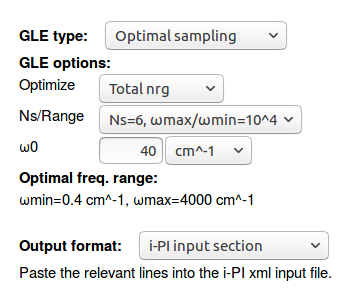
\includegraphics[width=\textwidth]{parameters_gle_2017.png}
\end{minipage}}

% \texttt{<dynamics mode="nvt">\\
%          <timestep units="femtosecond"> 0.5 </timestep>\\
%          <thermostat mode='gle'>\\
%            <A shape='(5,5)'>\\
%              [   1.119252684345e-2,    8.975945537096e-6,   -2.728650447177e-5,   -7.011051989908e-4,    8.414373543550e-3,
%           1.194065829660e-7,    1.071876106695e-6,   -9.439643019253e-6,   -1.329262116026e-5,   -2.667325152958e-6,
%           2.161979961890e-4,    9.439643019253e-6,    4.639122293442e-5,    4.329184279724e-6,    8.132076333400e-5,
%          -7.322257663569e-4,    1.329262116026e-5,   -4.329184279724e-6,    5.173717780694e-4,    1.590872642196e-5,
%           8.299189140989e-3,    2.667325152958e-6,   -8.132076333400e-5,   -1.590872642196e-5,    6.992095202254e-3
%             ]
%            </A>\\
%          </thermostat>\\
%       </dynamics>
% }

\item Colored noise thermostat

\begin{minipage}[l]{0.6\textwidth}
 
The parameters for this thermostat are quite complex. 
We will here use it to approximate nuclear quantum effects (that is, we will not simulate a canonical ensemble), 
so that the matrices $\mathbf{A}$ and $\mathbf{C}$ (Eq. \ref{eq:gle-eom}) will have to be given as an input. 
They can be generated at  
\href{http://gle4md.org/index.html?page=matrix}{http://gle4md.org/index.html?page=matrix}.\\
Choose the parameters in the website like it is shown in the picture, and copy them to the input.xml file.
\end{minipage}
\fbox{\begin{minipage}[r]{0.4\textwidth}
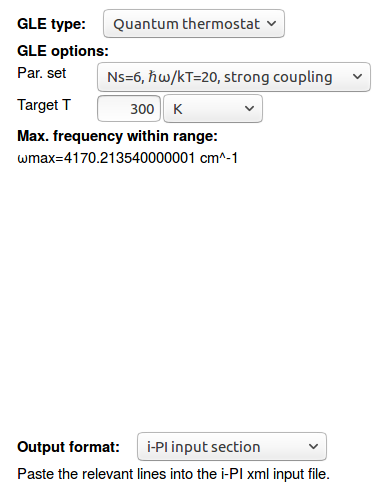
\includegraphics[width=\textwidth]{parameters_quantum_gle_2017.png}
\end{minipage}}

% \textt{  <thermostat mode='gle'>\\
%            <A shape='(7,7)'>\\
%              [   9.443659190019e-6,    1.132294186893e-3,    7.449628436962e-4,    1.071101169467e-3,    1.223429397683e-3,    6.267797080926e-4,    3.661966178600e-4,
%          -1.158486730163e-3,    4.928600223455e-4,    1.595931933797e-3,   -2.062890689123e-4,   -5.396142818401e-5,    1.594791295865e-4,   -1.609441915443e-3,
%          -7.027092008132e-4,   -1.595931933797e-3,    5.047934082853e-4,    2.770764198362e-4,    7.526274670274e-4,    2.664551238983e-4,   -7.897558467954e-4,
%          -1.072792654821e-3,    2.062890689123e-4,   -2.770764198362e-4,    5.772022515510e-4,    2.126703161982e-5,    7.244407882208e-4,    3.701736742286e-4,
%          -1.189347224241e-3,    5.396142818401e-5,   -7.526274670274e-4,   -2.126703161982e-5,    6.304868735244e-4,   -8.366171930319e-4,    2.357048551293e-3,
%          -3.148986705340e-4,   -1.594791295865e-4,   -2.664551238983e-4,   -7.244407882208e-4,    8.366171930319e-4,    5.722269541087e-3,   -7.870057326856e-3,
%          -7.265098725829e-4,    1.609441915443e-3,    7.897558467954e-4,   -3.701736742286e-4,   -2.357048551293e-3,    7.870057326856e-3,    9.273239517793e-3
%             ]
%            </A>\\
%            <C shape='(7,7)' units='kelvin'>\\
%              [   2.999985914100e+2,    5.937593337000e+0,    2.144376751500e+2,    5.883055908000e+1,   -1.119803766000e+2,   -6.793381764000e+1,    1.379789732400e+1,
%           5.937593337000e+0,    3.781851303000e+2,   -5.794518522000e+1,   -2.178772681500e+2,   -1.649310659100e+2,   -6.557113452000e+1,    3.833830743000e+1,
%           2.144376751500e+2,   -5.794518522000e+1,    7.325759985000e+2,    2.188507713000e+2,   -3.704586531000e+2,   -3.385193865000e+1,   -4.827706758000e+0,
%           5.883055908000e+1,   -2.178772681500e+2,    2.188507713000e+2,    6.960431520000e+2,   -3.630171093000e+2,    1.702940985000e+2,   -6.073265904000e+1,
%          -1.119803766000e+2,   -1.649310659100e+2,   -3.704586531000e+2,   -3.630171093000e+2,    1.437872295000e+3,    1.124747403900e+2,    3.533754279000e+0,
%          -6.793381764000e+1,   -6.557113452000e+1,   -3.385193865000e+1,    1.702940985000e+2,    1.124747403900e+2,    1.489339230300e+3,   -1.607601813300e+2,
%           1.379789732400e+1,    3.833830743000e+1,   -4.827706758000e+0,   -6.073265904000e+1,    3.533754279000e+0,   -1.607601813300e+2,    4.445083650000e+2
%             ]
%            </C>\\
%          </thermostat>\\
%        }

% \item Nos\'e-Hoover
% 
%  \texttt{MD\_run 1.0 NVT\_nose-hoover 300  $Q$}
% Hint: It can be shown (and is actually a fun exercise) that the optimal mass for the Nos\'e-Hoover thermostat is 
% $Q=3Nk_BT/\omega^2$, as shown in Ref. \cite{martyna-klein-tuckerman}. 
% Considering H$_5$O$_2^+$ (D$_5$O$_2^+$) has vibrational modes between  roughly 100 and 4000 cm$^{-1}$ (70 and 3000) cm$^{-1}$, which mass would you choose for the thermostat? %(but has a gap between 1500 and 2900cm$^{-1}$)
% %, derive an expression that links $Q$ with its (angular) frequency $\omega$ and estimate $Q$.
% More straightforwardly, the flag \verb, MD_thermostat_units cm^-1, can be used to input the thermostat mass directly in $cm^{-1}$.\\
% (A control file \texttt{control.nose-hoover\_programmed.in} with a reasonable value of Q is provided in \texttt{exercise\_2/solution/})
% %Answer: Q (amu * bohr$^2$) 1E-4 /(4 pi$^2$ amu c$^2$ bohr$^2$) 3Nk$_B$T/f$^2$ = 83.6818496904 3NT/f$^2$


% \item Bussi-Donadio-Parrinello (BDP)
% 
% \texttt{MD\_run  1.0  NVT\_parrinello 300  $\tau$}
% 
% Hint: Use $\tau$ (the unit is ps) equal to $\approx20$--$50$ time steps. 
% Unless $\tau$ is too small with respect to the time step (1--5 time steps), the actual value of $\tau$ does not affect the performance of this thermostat; 
% with a milder coupling, one observes a slower response to the imposed change of temperature, though.




\end{enumerate}

\item While waiting for the simulations to complete, you are challenged to demonstrate Eq.~\ref{eq:MBdistr} and calculate what would be the temperature 
corresponding to a zero point energy ($\hbar\omega/2$) for a frequency $\omega_1 = 3000$ cm$^{-1}$ and for $\omega_2 = 100$ cm$^{-1}$ considering a system with only 1 degree of freedom. 
Also show which frequency $\omega$ corresponds to a temperature of 300K.

%\item It can be shown that the optimal mass for the Nos\'e-Hoover thermostat is 
%$Q=3Nk_BT/\omega^2$, as shown in Ref.\cite{martyna}. 
%Considering H$_5$O$_2^+$ (D$_5$O$_2^+$) has vibrational modes between roughly 100 and 4000 cm$^{-1}$ (70 and 3000) cm$^{-1}$, 
%which mass would you choose for the thermostat? %(but has a gap between 1500 and 2900cm$^{-1}$)
%, derive an expression that links $Q$ with its (angular) frequency $\omega$ and estimate $Q$.
%Answer: Q (amu * bohr$^2$) 1E-4 /(4 pi$^2$ amu c$^2$ bohr$^2$) 3Nk$_B$T/f$^2$ = 83.6818496904 3NT/f$^2$


\item Use the script get\_properties.py to extract different properties, like the temperature, the kinetic energy and the potential energy:

\texttt{python get\_properties.py  `property' `ipi-output'}

where `property' is a placeholder for the property you want to extract. You can choose from `temperature', `kinetic', `potential' and`'conserved'.
This will output a single-column file containing the desired property at every step of the simulation.
Plot each of these quantity. Is it what you were expecting ?

\item Let us analyze a bit further the output.
Use the script \texttt{histogram} in order to obtain the temperature distribution of your system:

\texttt{histogram -xi 0 -xf 600 < mean\_temperature.dat > histo.dat}

(Here we assumed 'temperature.dat' is your single-column file containing the temperature of the system at each time step.)
What is the shape of the distribution ? Why ?

Another way to analyze the behavior of the temperature of your system is to look at the cumulative average, that is, the average temperature over time computed at each step of the simulation. You can do this by running the following script:

\texttt{python cumul\_avg.py `mean\_temperature.dat'}

Can we assert that the system is correctly thermalized ?

Now use the script ``autocorr'' to calculate the autocorrelation function of the potential energy:

\texttt{autocorr -maxlag 1000 < `potential.ex4.out.dat' > `autocorr.dat'}

Plot the autocorrelation function against time. What is the decorrelation time ? (How) does it change with respect to tau ?


\item Calculate the instantaneous temperature of each atomic species for each thermostat you tried by using the following script:

\texttt{python get\_temp\_species.py  `ipi-output' O H}

where `O' and `H' define the oxygen and hydrogen species. How do the different thermostats work in each case? 
Do the thermostats couple efficiently to the system?
Can you understand the result for the quantum thermostat? 
(Hint: different vibrational frequencies involve different atoms and give rise to different zero point energies)


\item The script ``get\_rdf\_h5o2.py'' writes the radial distribution function $g(r)$, decomposed into OH, OO, and HH pairs. Run the script on each \textbf{FHI-aims output} by typing:

\texttt{python get\_rdf\_h5o2.py  `output-aims'}

It will output three files, starting with `rdf\_oo', `rdf\_oh' and `rdf\_hh'. The first column is the distance (in \AA ngstroms) and the second column the count. Plot these files for each thermostat you used and compare the results for each $g(r)$.
%In the next exercise we will calculate the same data with path integral molecular dynamics, so that we can compare! 
For which $g(r)$ of you see the larger differences between the classical and ``quantum thermostat" distribution?
%Compare the $g(r)$ of H$_5$O$_2^+$ and D$_5$O$_2^+$ (the results for the cluster that you have not run are in \texttt{exercise\_4/solutions/}). Could you predict the differences? Can you understand them?

%\item In the folder \texttt{exercise\_2/solutions/} we provide the output files for 20ps long simulations (all three cases). You can compare with the simulations you have done.

\end{itemize}


\textit{Time estimation: $\sim$1h}

%%%%%%%%%%%%%%%%%%%%%%%%%%%%%%%%%%%%%%%%%%%%%%%%%%%%%%%%%%%%%%%%%%%%%%%%%%%%%%%%%%%%%%%%%%%%%%%%%%5555
\newpage
{\large\textbf{Exercise 5: Free energy estimation via Thermodynamic Integration.}}


\begin{wrapfigure}{r}{0.45\textwidth}
\begin{center}
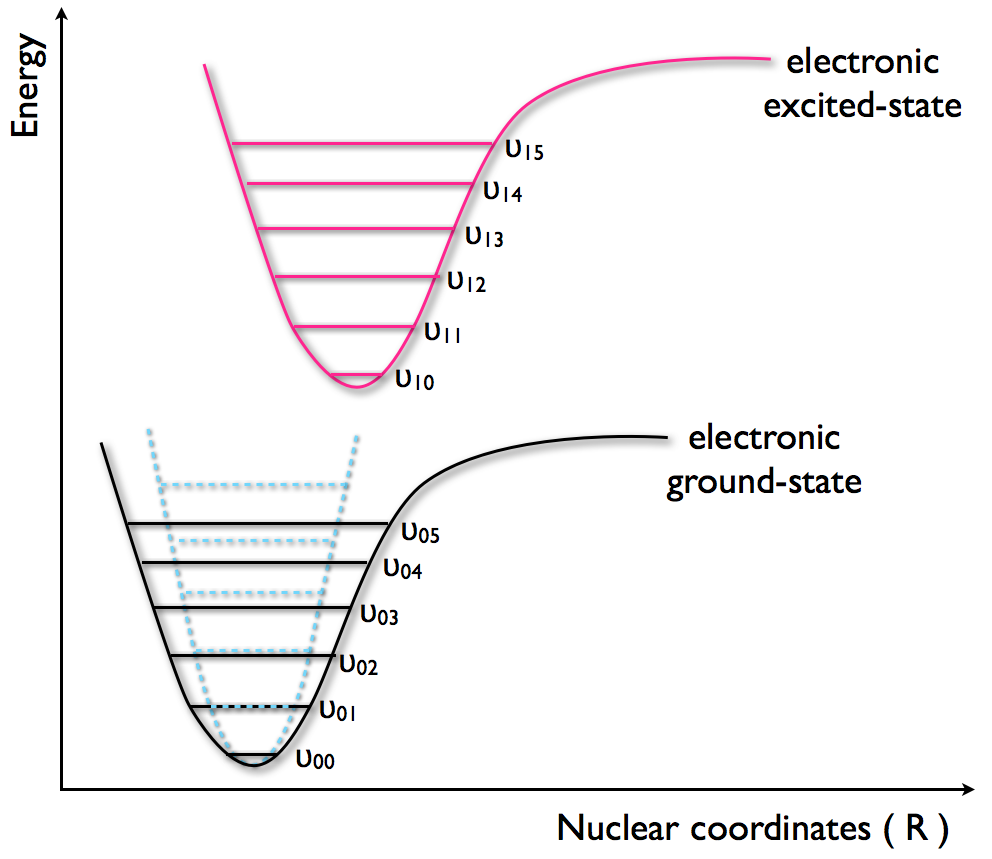
\includegraphics[width=0.44\textwidth]{vibrations_pic.png}
\caption{Schematic drawing of electronic and vibrational states of a hypothetical molecule. The Morse-like curves in black and pink represent the electronic
ground-state and the first excited state, respectively. The levels drawn in each of them correspond to the possible vibrational frequencies $v_{0n}$, $v_{1n}$.
The dashed parabola-like blue line represents the harmonic approximation, with equally spaced vibrational levels. \label{fig:vibs}}
\end{center}
\end{wrapfigure}

While the potential energy surface is shaped by the 3$N$ coordinates (degrees of freedom)
that describe a molecule, the \textit{free} energy, which is the quantity
actually accessible in experiments, is a function of thermodynamical variables (temperature,
pressure, entropy, volume, etc.).
This is the quantity of fundamental interest for comparison with experiments
and the one that rules all dynamics of the system.
In order to perform the task of calculating free energies, it is necessary to define
the partition function $Z(T)$ of the system of interest.
With respect to the canonical partition function $Z(T)$,
the Helmholtz free energy can be written as \cite{mcquarrie}:

\begin{equation}
F (T) = -k_B T \ln [Z(T)], %= -k_B T ln \left( \sum_\zeta g(\zeta) e^{-\frac{\zeta}{k_B T}} \right), 
\label{eq:free_energy_compact}
\end{equation}

\noindent where $k_B$ is the Boltzmann constant and $T$ is the temperature.



In the harmonic-oscillator approximation,
the  partition function can be
written as a product of the several vibrational energy levels,
weighted according to the Bose-Einstein statistics to take
into account the quantum nature of the nuclei


\begin{equation}
Z_{\text{vib}}^{\text{ha}}(T)=\prod_{i=1}^{3N-6} \frac{e^{-\frac{\hbar \omega_i}{2k_B T}}}{1-e^{-\frac{\hbar \omega_i}{k_B T}}},
\label{eq:part_func_osc}
\end{equation}

\noindent where $\omega_i$ are the normal modes of vibration of the molecule and the product runs over all modes except the ones corresponding to translations and rotations \footnote{One can also include the contributions to the partition function and the free energy arising from rotations and translations (see Ref. \cite{mcquarrie} for possible approximations for these quantities), and in real systems these may not even be separable. In this exercise we will focus on only vibrational contributions, though.}. Substituting \ref{eq:part_func_osc} in \ref{eq:free_energy_compact}, we get the following expression for the vibrational
contributions to the harmonic free energy, $F^{\text{ha}}_{\textit{vib}} (T)$:
\begin{equation}
F^{\text{ha}}_{\textit{vib}} (T) = \sum_{i=1}^{3N-6} \left[ \underbrace{\frac{\hbar \omega_i}{2}}_{\text{Zero Point Energy}} + k_B T \ln\left(1-\exp^{-\frac{\hbar \omega_i}{k_B T}}\right)\right].
\label{eq:free_energy}
\end{equation}

There are limitations to the use of the harmonic approximation. It is not expected to be valid at all temperatures, due to its harmonic nature:
When the atoms start to explore higher regions of the potential well, it cannot be approximated
as a parabola. The ``real'' anharmonic modes are more closely spaced than what is estimated by the harmonic approximation, as can be pictorically seen in Figure \ref{fig:vibs}.
% On the other hand, for very low temperatures and light molecules, the premise that the system 
% follows Boltzmann statistics (number of available states much greater than number of particles) does not hold, and the 
% calculation of the partition function becomes very involved \cite{mcquarrie}.
One way to obtain anharmonic corrections to the harmonic free-energy
will be the subject of this exercise.

From elementary thermodynamics, in the canonical (NVT) ensemble, one can write
\begin{align} \label{eq:difffe}
 \frac{\partial \left( \beta F \right) }{\partial \beta} = \left\langle U \right\rangle_{NVT},
\end{align}
\noindent where $\beta=1/(k_B T)$, $F$ is the Helmholtz free energy, and ${U}$ is the internal energy (potential plus kinetic energy) of the system
and the brackets $\left\langle \ldots \right\rangle_{NVT}$  denote the canonical average. We can then evaluate the free energy at a temperature $T$ by integrating Eq. \ref{eq:difffe}

\begin{eqnarray} \label{eq:febeta1}
\frac{F(T)}{k_B T} & =  & \frac{F_0(T_0)}{k_B T_0} + \int_{\beta_0}^{\beta} d \beta' \langle U \rangle_{\beta'}, 
% & = & \frac{F_0(T_0)}{k_B T_0} - \frac{1}{k_B} \int_{T_0}^{T} d T' \frac{\left\langle U \right\rangle_{T'}}{T'^2} 
 \end{eqnarray}

\noindent where $F_0(T_0)$ is the free energy at a reference temperature. The term $ \langle U \rangle_{\beta'}$ can be written as a sum of two contributions, namely,

\begin{equation}\label{eq:def_an}
\langle U \rangle_{\beta} = \langle U^{\text{ha}}\rangle_{\beta} + \langle \Delta U^{\text{an}} \rangle_{\beta}, 
\end{equation}

\noindent where $\langle \Delta U^{\text{ha}} \rangle_{\beta}$ is the ensemble average of the harmonic contributions to the internal energy (which we know how to solve analytically) and $\langle \Delta U^{\text{an}} \rangle_{\beta}$ 
is the ensemble average of the anharmonic contributions.
 
So far, all the  presented equations are exact. In practice, the integral in Eq. \ref{eq:febeta1} is evaluated numerically by sampling $\langle U \rangle_{\beta}$ for a discrete set of temperatures from $T_0$ to the desired $T$. Then, a numerical integration can be performed. Now we make an approximation, namely that our system can be approximated as harmonic at $T_0$, so that $F_0(T_0) \approx F_0^{ha}(T_0)$. This approximation is best when $T_0$ is a low temperature. Then, one can use equations \ref{eq:febeta1} and \ref{eq:def_an} to write 

\begin{equation}
F(T) = F^{\text{ha}}_{\textit{vib}}(T) + k_B T \int_{\beta_0}^{\beta} d\beta' \langle \Delta U^{\text{an}} \rangle_{\beta'},
\label{eq:anharm-correction}
\end{equation}


\noindent where $F^{\text{ha}}_{\textit{vib}}(T)$ is given by equation \ref{eq:free_energy}.\footnote{The careful reader will realize that the free energy in Eq. \ref{eq:anharm-correction} is the total free energy and not the vibrational one. This is because the second term in the right hand of that equation includes the rotational contribution. However, a term is still missing. We neglect it for simplicity and it does not change any conclusion to this exercise. If you are so curious that you have reached this point, could you guess which term is it before that you continue reading?\\
Find the answer in the reference \cite{answer}  }


 We will consider two approaches to evaluate the ensemble average of $\Delta U^{\text{an}}$.
First, we will consider MD simulations with classical nuclei as we did in the previous exercises. 
Then, we will use path integral molecular dynamics (PIMD). As was discussed in the lecture, PIMD is classical molecular dynamics in an extended space:
Each quantum particle is mapped onto a ring polymer of classical particles, which consists of $n$ repetitions of the original system connected by harmonic springs. This method thus increases the cost of the calculation by $n$. Since the
harmonic forces of the springs are easily and analytically evaluated, the method is also trivially parallelizable.
Note that in the first case we make a further approximation, where we consider the anharmonic contributions
in a classical framework, but add their effect to the ``quantum'' harmonic free energy
of equation \ref{eq:free_energy}.

Also, in this exercise we will use an interesting feature of i-PI, which is that several different clients can be connected to it, and they do 
not need to be electronic structure codes. In this case, we will use the \texttt{driver.x} code, which is distributed with i-PI and has many empirical or parametrized potentials coded into it. We will be using the potential from Ref. \cite{bowman}, that was parametrized on a calculated CCSD(T) surface for the Zundel cation, and provides much faster force evaluations than solving explicitly the Kohn-Sham equations as we were doing until now.

Finally, instead of providing you one file that performs all the post processing like a black box,
we provide you several scripts ({\texttt{exercise\_5/scripts/}}) that perform specific tasks so you understand the procedure step by step:
\begin{enumerate}



\item { \texttt{F\_ha.py} }
  \begin{itemize}
    \item{ \textbf{Function:} Computes the vibrational Helmholtz free energy up to a given temperature within the harmonic approximation}
    \item{ \textbf{Syntax:} \texttt{ python proc.py <InputFreq\_file> <Max\_Temperature>} }
    \item{ \textbf{Input:} The <InputFreq\_file> is the name of the file with the frequencies list (provided) }
  \end{itemize} 


\item { \texttt{U\_ha.py} }
  \begin{itemize}
    \item{ \textbf{Function:} Computes the total internal energy (classical and quantum) up to a given temperature within the harmonic approximation}
    \item{ \textbf{Syntax:} \texttt{ python proc.py <Input\-Freq\_file> <Max\_Temperature>} }
    \item{ \textbf{Input:} The <Input\_Freq\_file> is the name of the file with the frequencies list (provided) }
  \end{itemize} 


\item {\texttt{extract\_mean.py}}
  \begin{itemize}
    \item{ \textbf{Function:} Computes averages value and standard deviation from an i-PI output file }
    \item{ \textbf{Syntax:} \texttt{ python proc.py <name\_input>  <mode>} }
    \item{ \textbf{Mode options:} T (temperature), V (potential energy), K (Kinetic energy), K+V (Internal energy, U = K+V) }
    \item{ \textbf{Input}: i-PI output file }
  \end{itemize}
  
\item {\texttt{integrate.py}}
  \begin{itemize}
    \item{\textbf{Function:} Computes the second term of the equation \ref{eq:anharm-correction} including the $k_B T$ factor }
    \item{\textbf{Syntax:} \texttt{python proc.py <name\_input>  <number of points>} }
    \item{\textbf{Input:} Two columns format. First column corresponds to the temperature and second column corresponds to $\left\langle \Delta U^{\text{an}} \right\rangle_{\beta}$. (Every line starting with \# is discarded )}
  \end{itemize}  

\end{enumerate}

 
\noindent{\textbf{ Instructions}}
\begin{itemize}
\item{Look at the folder \texttt{exercise\_5/data/}. There you can find three files: \texttt{MD.dat}, \texttt{H5O2\_PIMD.dat} and \texttt{D5O2\_PIMD.dat}. (Why do we not specify \texttt{H5O2\_MD.dat} or \texttt{D5O2\_MD.dat} ?). Open one of them. You will see the data in two columns. The first one is the temperature  $T$(K)  and the second one the anharmonic contribution to the average internal energy  $\left\langle \Delta U^{\text{an}} \right\rangle_{\beta}$. You will notice that the table is not complete, your job is to complete it.}
\item{Again, in order to speed up the exercise, each group will simulate either H$_5$O$_2^+$ or D$_5$O$_2^+$. The suggested choice of the molecule will be made clear (announced) by the tutors at hand.}

\item{In order to compute the missing values you have to run MD or PIMD simulations. We provided the corresponding templates in the folder
\texttt{exercise\_5/skeleton/}. In particular, we provided one \texttt{input.xml} and one checkpoint file with an equilibrated geometry for each simulation. Please take your time in order read and understand the \texttt{input.xml} files: Which differences can you identify? Do you understand them?}

\item{Here is how you will run i-PI and the \texttt{driver} code with the parametrized potential for the Zundel cation:}


\vspace{0.3cm}
\colorbox{Apricot}{\frame{\begin{minipage}[r]{0.95\textwidth}
\vspace{0.3cm}
\begin{center}
In order to start  the simulation type:\\

\vspace{0.3cm}
\texttt{\IPI \, > output-i-PI \&}\\
\vspace{0.3cm}
(Wait 5 seconds in order to let i-PI do the initialization)\\
\vspace{0.3cm}
Open a second terminal and start:\\
\vspace{0.3cm}
\texttt{driver.x -u -m zundel -h <address> \& }

\begin{itemize}
\item ATTENTION: the \texttt{<address>} in the previous command MUST coincide\\
with the address specified in the i-PI input file. 

\item For PIMD simulations you can (should) run several instances of the client at the same time. That way each replica of your system will be calculated by different instances of the \texttt{driver} code. In order to do that please run 

\texttt{for i in \{1..8\}; do driver.x -u -m zundel -h <address> > out\_\$i \&   done}

\texttt{ }

\end{itemize}
\vspace{0.3cm}
\end{center}
\end{minipage}}}

\item{Go to \texttt{exercise\_5/skeleton/1\_MD/200K} and run the MD simulation. Then, go to \texttt{2\_H5O2\_PIMD/300K/} or \texttt{3\_D5O2\_PIMD/250K/} and run the PIMD simulation. 
\textbf{You can run both simulations at the same time.}}
\item{{\em During the waiting time of this exercise, you may try to demonstrate Equation \ref{eq:anharm-correction}}}.
\item{When all the simulations are over, you have to do the post processing}
\item{Use the provided script \texttt{extract\_mean.py} to compute the averages of internal energy for each simulation}
\item{Use the provided script  \texttt{U\_ha.py} to compute the internal energy in the harmonic approximation. Since the MD simulations treat the nuclei as \textit{classical} particles, the reference internal energy must be the harmonic classical energy, given by the equipartition theorem $U^{\text{ha}}(T)= {(3N-6)}k_BT$. For the PIMD case the reference internal energy must be the quantum harmonic internal energy. Luckily the script provides you both of them, so take the appropriate value for each case.}
\item{Calculate the $\left\langle \Delta U^{\text{an}} \right\rangle_{\beta}$ (equation \ref{eq:def_an}) and complete the tables}
\item{ Use the provided script \texttt{F\_ha.py} to compute the Harmonic Free energy, $F^{\text{ha}}_{\text{vib}}(T)$}
\item{ Use the provided script \texttt{integrate.py} to perform the integrations . Remember that with the integration you are getting the anharmonic corrections, so to get the total free energy, $F(T)$, you have to add the harmonic contribution (equation \ref{eq:anharm-correction})}

\item{ Plot $F(T)$  and $F^{\text{ha}}_{\text{vib}}(T)$ as a function of temperature (in xmgrace, for example) }



\vspace{0.3cm}
What are the differences? Can you estimate up to which temperature the harmonic approximation should be a good approximation? Are the anharmonicities important for these systems? And the nuclear quantum effects?




\item Fun question if you want to try at home: Can you reproduce the result obtained with PIMD by instead performing MD with classical nuclei but employing the quantum thermostat of the previous exercise?

\end{itemize}






\textit{Timing: $\approx$1h20min total}

\clearpage



%################################################################################
\begin{thebibliography}{50}
\bibitem{ipi} \href{https://doi.org/10.1016/j.cpc.2013.10.027}{M. Ceriotti, J. More, D. E. Manolopoulos, Comput. Phys. Comm. \textbf{185} 1019 (2013).}
\bibitem{Feynman} R. P. Feynman, and A. R. Hibbs \textit{Quantum Mechanics and Path Integrals}; McGraw-Hill: New York, 1965.
\bibitem{frenkel-smit} D. Frenkel and B. Smit, \textit{Understanding Molecular Simulation: from algorithms to applications}, second edition, Academic Press 2002.
\bibitem{bdp} \href{http://dx.doi.org/10.1063/1.2408420}{G. Bussi, D. Donadio, and M. Parrinello, J. Chem. Phys. \textbf{126}, 014101 (2007).}
\bibitem{andersen} \href{http://dx.doi.org/10.1063/1.439486}{H. C. Andersen, J. Chem. Phys. \textbf{72}, 2384 (1980).}
\bibitem{berendsen} \href{http://dx.doi.org/10.1063/1.448118}{H. J. C. Berendsen et al., J. Chem. Phys. \textbf{81}, 3684 (1984).}
\bibitem{tuckerman} M. E. Tuckerman, \textit{Statistical Mechanics: Theory and Molecular Simulation}; Oxford University Press 2010. 
\bibitem{ceriotti10} \href{http://pubs.acs.org/doi/abs/10.1021/ct900563s}{M. Ceriotti, G. Bussi, and M. Parrinello, J. Chem. Theory Comput. \textbf{6}, 1170 (2010).}
\bibitem{nosehoover} \href{http://dx.doi.org/10.1063/1.447334}{S. Nos\'{e}, J. Chem. Phys. \textbf{81}, 511 (1984).} \href{https://doi.org/10.1103/PhysRevA.31.1695}{W.G. Hoover, Phys Rev. A \textbf{31}, 1695 (1985).}
\bibitem{martyna} \href{https://doi.org/10.1063/1.463940}{G. Martyna, M. Klein, and M. Tuckerman,  J. Chem. Phys.\textbf{97} 2635 (1992).}
\bibitem{mcquarrie} D. McQuarrie, \textit{Statistical Mechanics}, University Science Books, 1st. ed., (2000).
\bibitem{bowman} \href{http://aip.scitation.org/doi/10.1063/1.1927529}{X. Huang, B. J. Braams, and J. M. Bowman, J. Chem. Phys. \textbf{122}, 044308 (2005).}
\bibitem{answer} The answer is the rotational contribution at $T_0$.
%YL This is the answer for a footnote question in the exercise 5
%\bibitem{Newton} I. Newton, {\em Philosophi\ae{} Naturalis Principia Mathematica}, London (1687)
%\bibitem{Kolafa1996} J. Kolafa,  Mol. Simul. \textbf{18}, 193 (1996)
%\bibitem{KuehneParrinello2007} K\"uhne, Thomas D. \textit{et al}., Phys. Rev. Lett. \textbf{98}, 066401 (2007)
%\bibitem{niklasson-challacombe} A. M. N. Niklasson, C. J. Tymczak, and M. Challacombe, Phys. Rev. Lett. \textbf{97}, 123001 (2006)
%\bibitem{arias-joannop} T. A. Arias, M. C. Payne, and J. D. Joannopoulos, Phys. Rev. B \textbf{45}, 1538 (1992)
%\bibitem{niklasson} A. M. N. Niklasson, Phys. Rev. Lett. \textbf{100}, 123004 (2008)
%\bibitem{ishida} H. Ishida \textit{et al.}, Chem. Phys. Lett. \textbf{282}, 115 (1998)
%\bibitem{colored} M. Ceriotti, G. Bussi, M. Parrinello, JCTC \textbf{6}, 1170 (2010)\\ \texttt{https://epfl-cosmo.github.io/gle4md/}
%\bibitem{martyna-klein-tuckerman} G. Martyna, M. Klein, M. Tuckerman,  J. Chern. Phys. {\textbf 97}, 2635 (1992)
%\bibitem{piglet} M. Ceriotti, D. E. Manolopoulos, PRL \textbf{109}, 100604 (2012)
%\bibitem{gaigeot} M-P. Gaigeot, M. Martinez, and R. Vuilleumier, Mol. Phys. \textbf{105}, 2857 (2007)
%\bibitem{borysow-fromm} J. Borysow, M. Moraldi, and L. Frommhold, Molec. Phys. \textbf{56}, 913 (1985)
%\bibitem{ramirez-marx} R. Ramirez, T. Lopez-Ciudad, P. Kumar, and D. Marx, J. Chem. Phys. \textbf{121}, 3973 (2004)
% \bibitem{gaigeot} M-P. Gaigeot, M. Martinez, and R. Vuilleumier, Mol. Phys. \textbf{105}, 2857 (2007)
% \bibitem{borysow-fromm} J. Borysow, M. Moraldi, and L. Frommhold, Molec. Phys. \textbf{56}, 913 (1985)
% \bibitem{ramirez-marx} R. Ramirez, T. Lopez-Ciudad, P. Kumar, and D. Marx, J. Chem. Phys. \textbf{121}, 3973 (2004)
% \bibitem{mcquarrie} D. McQuarrie, \textit{Statistical Mechanics}, University Science Books, 1st. ed., (2000)
% \bibitem{SKE} T. M. Gibbons and S. K. Estreicher, Phys. Rev. Lett. \textbf{102}, 255502 (2009).
% \bibitem{AsMe} N. W. Ashcroft and N. D. Mermin, {\it Solid State Physics}, Cengage Learning, (1976).
\end{thebibliography}
\clearpage
%%%%%%%%%%%%%%%%%%%%%%%%%%%%%%%%%%%%%%%%%%%%%%%%%%%%%%%%%%%%%%%%%%%%%%%%%%%%%%%%%%%%%%%%%%%%%%%%%%%%%%%%%%




\appendix
\section{Plotting files in xmgrace}

In order to plot files containing multiple Y columns, follow these steps:

\begin{enumerate}
\item Open xmgrace and click on Data $\rightarrow$ Import $\rightarrow$ ASCII (Figure \ref{xmgrace1}).
\item Find the file that you want to plot and choose ``Load as Block Data'' in the dialogue box that will open (Figure \ref{xmgrace2}).
\item Set X from column 1 and Y from whatever other column you want to plot in the new dialogue box that will open (Figure \ref{xmgrace3}).
\item Press Apply and then press Close on all dialogues.
\end{enumerate}

Properties of the plots can be changed by double clicking on the data or on the axis.

\begin{figure}[ht]
\begin{center}
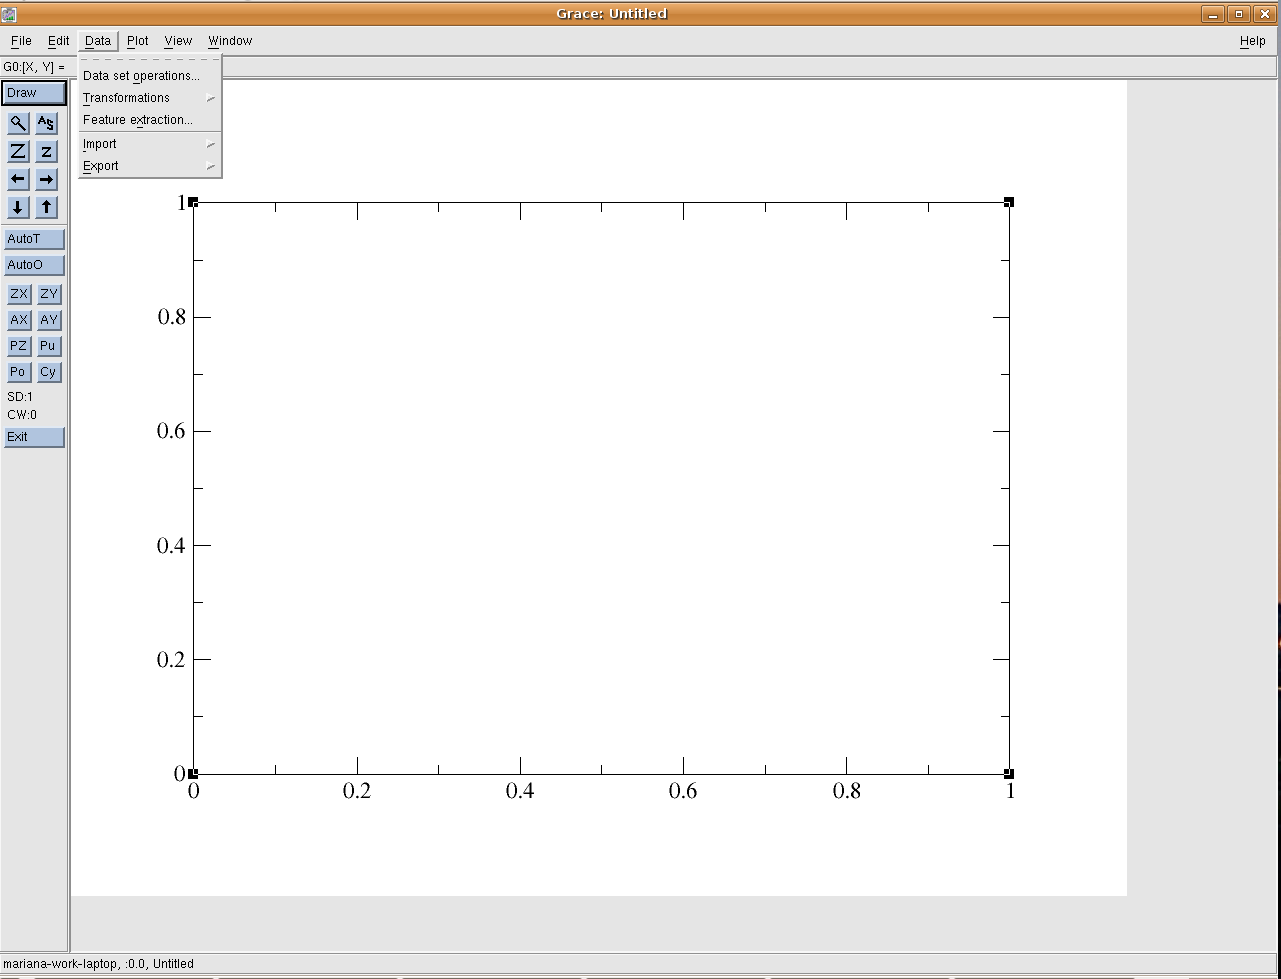
\includegraphics[width=0.7\textwidth]{xmgrace1}
\caption{Step 1 - Open xmgrace and click on Data $\rightarrow$ Import $\rightarrow$ ASCII}
\label{xmgrace1}
\end{center}
\end{figure}

\begin{figure}[ht]
\begin{center}
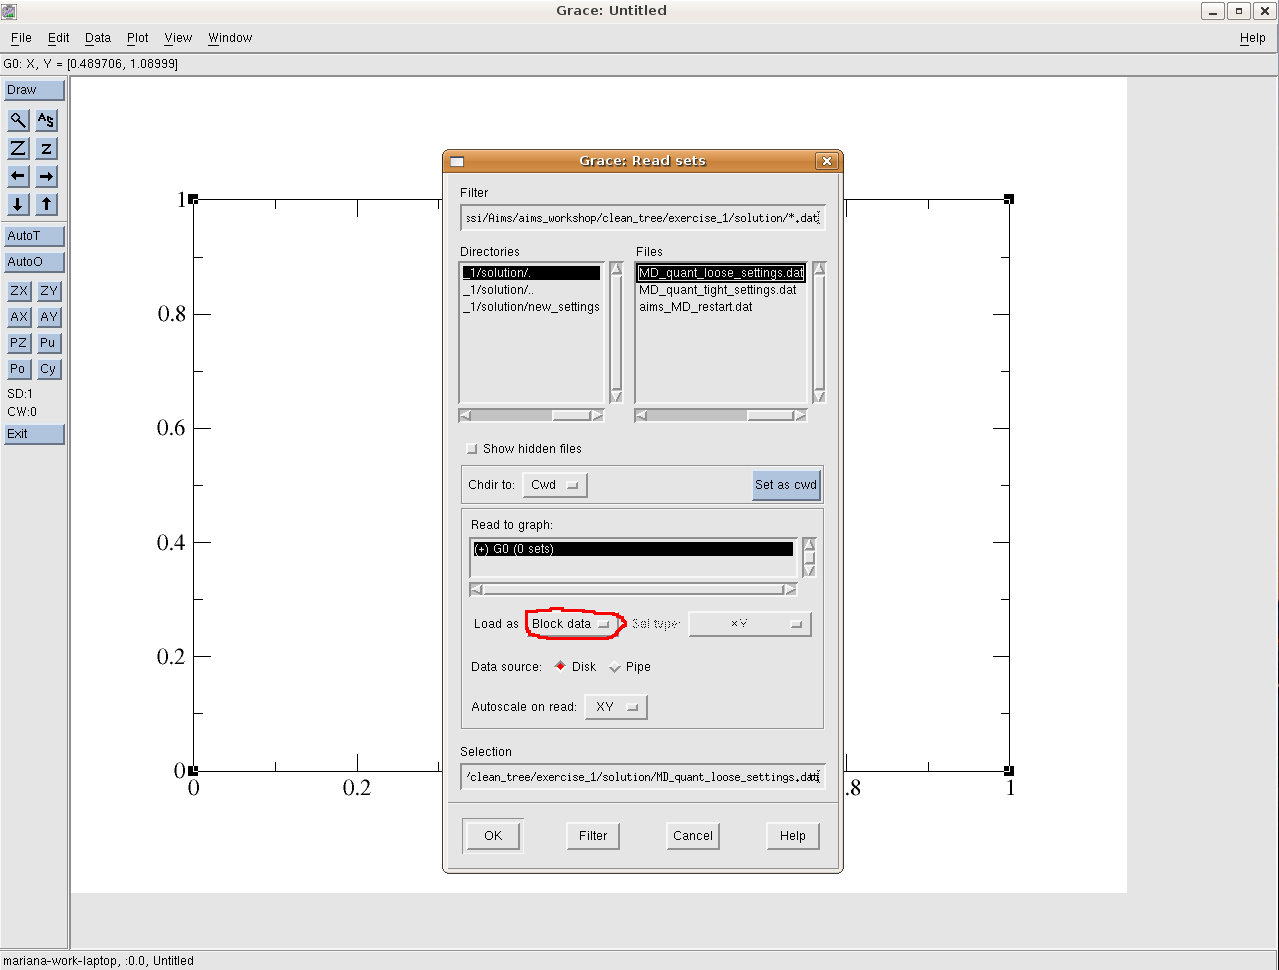
\includegraphics[width=0.7\textwidth]{xmgrace2}
\caption{Step 2 - Find the file that you want to plot and choose ``Load as Block Data'' in the dialogue box that will open.}
\label{xmgrace2}
\end{center}
\end{figure}

\begin{figure}[ht]
\begin{center}
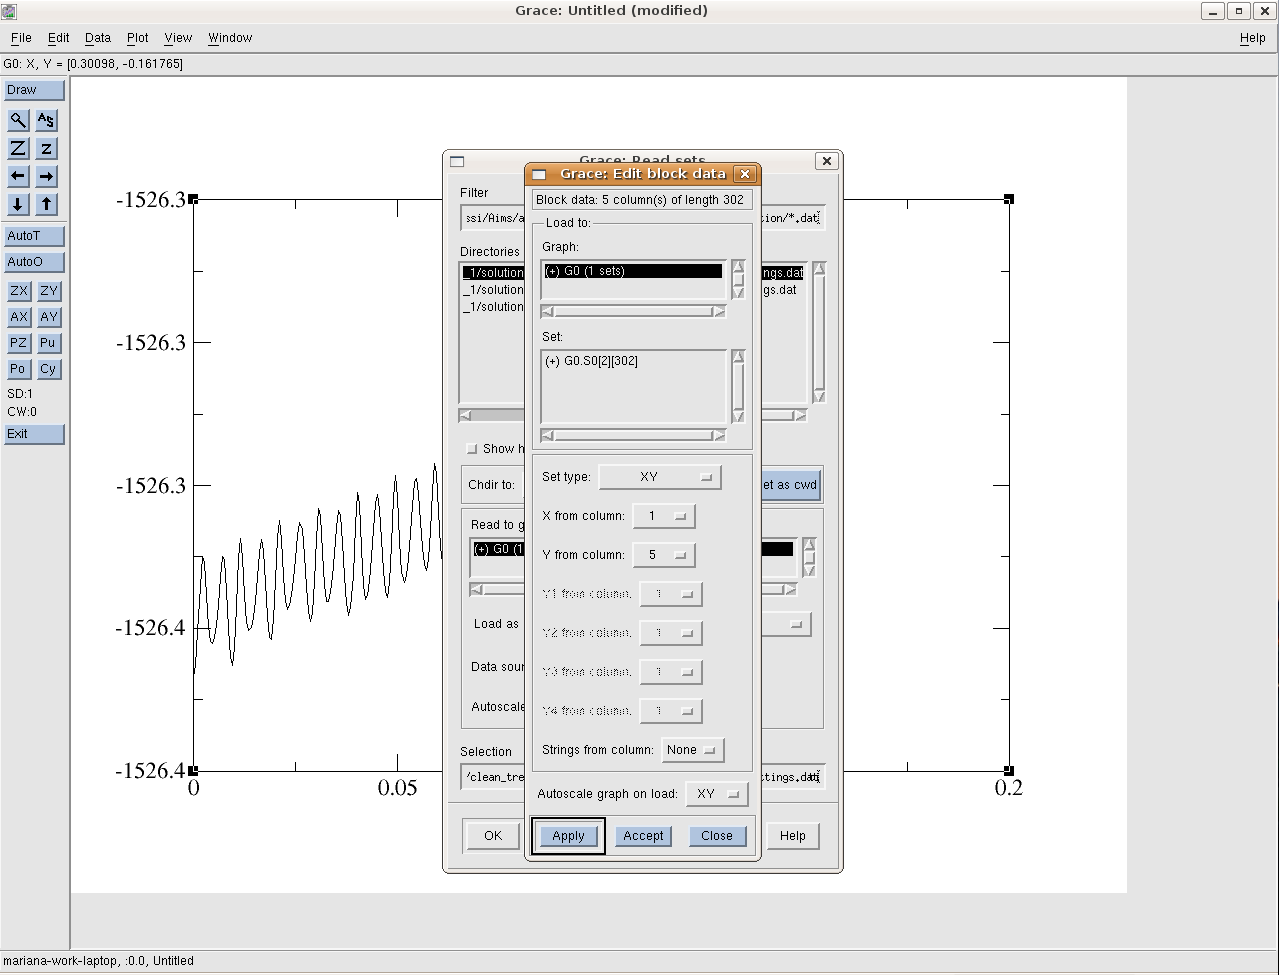
\includegraphics[width=0.7\textwidth]{xmgrace3}
\caption{Step 3 - Set X from column 1 and Y from whatever other column you want to plot in the new dialogue box that will open.}
\label{xmgrace3}
\end{center}
\end{figure}


\end{document}
%%%%%%%%%%%%%%%%%%%%%%%%%%%%%%%%%%%%%%%%%%%%%%%%%%%%%%%%%%%%%%%%%%%%%%%%%%%%%%%%%%%%%%%%%%%%%%%%%%%%%%%%%%






Here we will use the i-PI \cite{ipi} program in order to manage the calculation of the several replicas of the system,
that will, in turn, be simulated by FHI-aims.
The i-PI program works through a client-server architecture, where i-PI is the server that provides the evolution of the
equations of motion that sample the desired ensemble, and the \textit{ab initio} code (in this case FHI-aims) is the
client that provides the calculation of interatomic forces. i-PI uses internet or unix sockets, that allow the replicas of the system to be
simulated all in the same machine, in different nodes of one machine, or in different machines, as long as all the
calculations can communicate with the server.

The quantum properties of the system converge with the number of beads. Typically the number of beads needed is of the order of $\hbar \omega_{max}/k_B T$, where $T$ is the temperature being simulated and $\omega_{max}$ is the maximum frequency of vibration of the system.

One should always check the convergence of a property of interest before doing a PIMD calculation, but there will be no time for this in this exercise. Instead, in Figure  the average potential energy $\langle V \rangle$ and the average virial estimator for the kinetic energy $ \langle K_{cv} \rangle$ are given for H$_5$O$_2^+$ at 300K with LDA (like in the previous exercises). The expressions for these quantities in the PIMD formalism for a system of $n$ beads and $N$ particles are

\begin{eqnarray}
\langle V \rangle =\frac{1}{n}\sum_{i=1}^n \langle V(\textbf{ q}_i^1, ... , \textbf{ q}_i^N) \rangle \\
\langle K_{cv} \rangle = \frac{3 N k_B T}{2} + \frac{1}{2n} \sum_{j=1}^N\sum_{i=1}^n \langle ({\textbf{ q}}_i^j - \bar{\textbf{ q}}^j) \cdot \nabla V({\textbf{ q}}_i^1, ... , {\textbf{ q}}_i^N) \rangle
\end{eqnarray}

\noindent where $\bar{\textbf{ q}} = 1/n \sum_i {\textbf{ q}}_i $  is the position of the centroid. In Fig.
one sees that up to 64 beads (64 replicas of the system) are necessary to fully converge the quantities. This would be prohibitive for the use with first principles potential energy surfaces. One way to reduce the number of beads necessary to converge static (average) properties is to attach properly tuned thermostats based on the generalized langevin equation to the beads of the ring polymer, as proposed in Ref. \cite{piglet}. This is what is shown in red in Fig. , where one achieves convergence already with 8 replicas. Due to the computational resources available, we will only be able to perform calculations with 4 beads.

\begin{itemize}

\item \textit{Server:} An example of an input file for i-PI can be found inside the \texttt{exercise\_3/} folder, called
\texttt{input.xml}. It is an xml file, which is quite intuitive to learn. The input is not complete. Please take your time to
understand the keywords that are there and consult the i-PI manual found in \texttt{\$HANDSON/doc/manual.pdf}.

Besides setting the number of beads (4), there are two other fields that should be completed in the file: The field address about the socket communication and the field of the thermostat.

\begin{enumerate}
\item We will be using UNIX domain sockets here, since we will be running both server and client in the same machine. Just write in the \texttt{<address>} field a string of your choice, e.g. ipam-2014-h5o2 .
In the input there is a commented block with an example of how it would look if we would use internet sockets communicating with the local host. If using in different machines or nodes, one would have to give a proper IP address at the "address'' field.

\begin{minipage}[l]{0.55\textwidth}
\item The thermostat parameters can be found in \texttt{https://epfl-cosmo.github.io/gle4md/}. Choose the parameters in the website like it is shown in the picture and paste it into the relevant section of the i-PI input file. \end{minipage}
\fbox{\begin{minipage}[r]{0.35\textwidth}
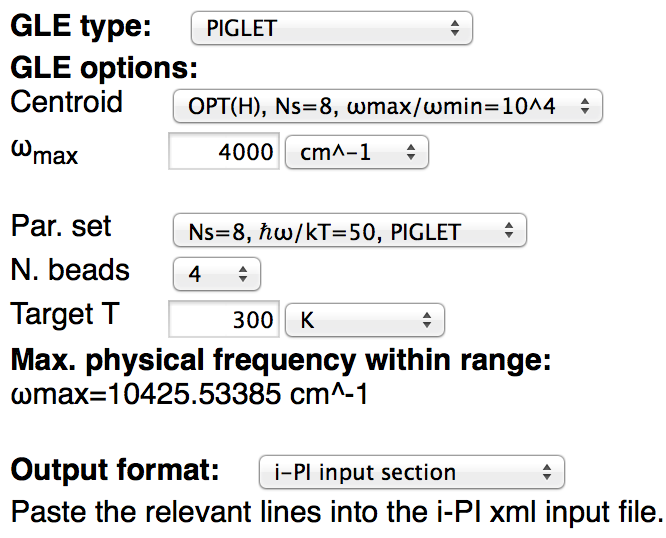
\includegraphics[width=\textwidth]{parameters_piglet_4beads.png}
\end{minipage}}
\end{enumerate}

More detailed instructions about the input file can be found in manual of i-PI, in Sec. 5.1.2.


\item \textit{Client:} The keyword to add to the \texttt{control.in} file that is in the \texttt{exercise\_3} folder of FHI-aims is \\
\texttt{use\_pimd\_wrapper hostaddress portnumber} \\
where hostaddress should be substituted by the address (IP or name) of the server and portnumber by the number of the port with which it should communicate. Since we are using UNIX domain sockets, one can just put a dummy number on the \texttt{portnumber} field. In the \texttt{hostaddress}  field write, for example, \texttt{UNIX:ipam-2014-h5o2}, i.e., the only constrain is that the string after the colon matches the \texttt{address}  field in the i-PI input file.

\item Launch the server by typing:

\texttt{python \$HANDSON/ipi/i-pi input.xml > out \&}

\item Launch four instances of FHI-aims by typing:

\texttt{for i in \{1..4\}; do (\$HANDSON/bin/aims.ipi.x > aims\$\{i\}.out \&) ; done}

\item When the simulation is done, run the script ``get\_rdf\_h5o2\_PI.py" to compute the radial distribution function $g(r)$ in the directory where the output files are, by typing:

\texttt{python get\_rdf\_h5o2\_PI.py piglet-h5o2 4}

where the first field is the prefix of the position files of all the beads and the second field is the number of beads.

\item Compare the $g(r)$ obtained here with the one from the previous exercises. For which species do you see most differences between the classical and the quantum case? Can you explain these results? (The simulation here may take a long time, but you can look at the rdf's while the simulation is running.)

\item While the simulation is running take your time to read the introduction of the i-PI manual, which explains in detail the architecture of the code and its capabilities.

\end{itemize}

\vspace*{24pt}
{\em In case you like to get challenged by a statistical mechanics question during the waiting time of this exercise, you may try to demonstrate that
the theoretical relative standard deviation of the temperature in the canonical ensemble is $\frac{\sigma^2}{T^2} = \frac{2}{3N}$.}

\clearpage
